\chapter{Publication}

The main steps of our approach are illustrated in \figref{fig:Apparatus}; a \ac{VHR} orthorectified image is provided and a the approximate trajectory of a sidewalk is acquired from a \ac{GIS} such as \ac{OSM}. Alternately, an approximate trajectory could be marked by a person to digitize the sidewalk quickly. The initial trajectory is re-sampled and used to warp a portion of aerial image so that the trajectory is mapped to a straight, horizontal line which we call a \textit{ribbon image}.  We use a modest assumption that colors near the center of the ribbon image are more likely to be on a walking path in order to build a probability-density estimate for walking path materials. Based on the probability estimate at each pixel, we construct a single ribbon with priors that control the rate of change of thickness and direction of the ribbon. Finally, the boundaries are warped back onto the original reference frame. In this section we elaborate the process of generating a ribbon image, estimating the probability that a color belongs to the same material as a walking path, and the construction of a smooth ribbon image based on the resulting probabilities. 

\begin{figure}[H]
\begin{center}
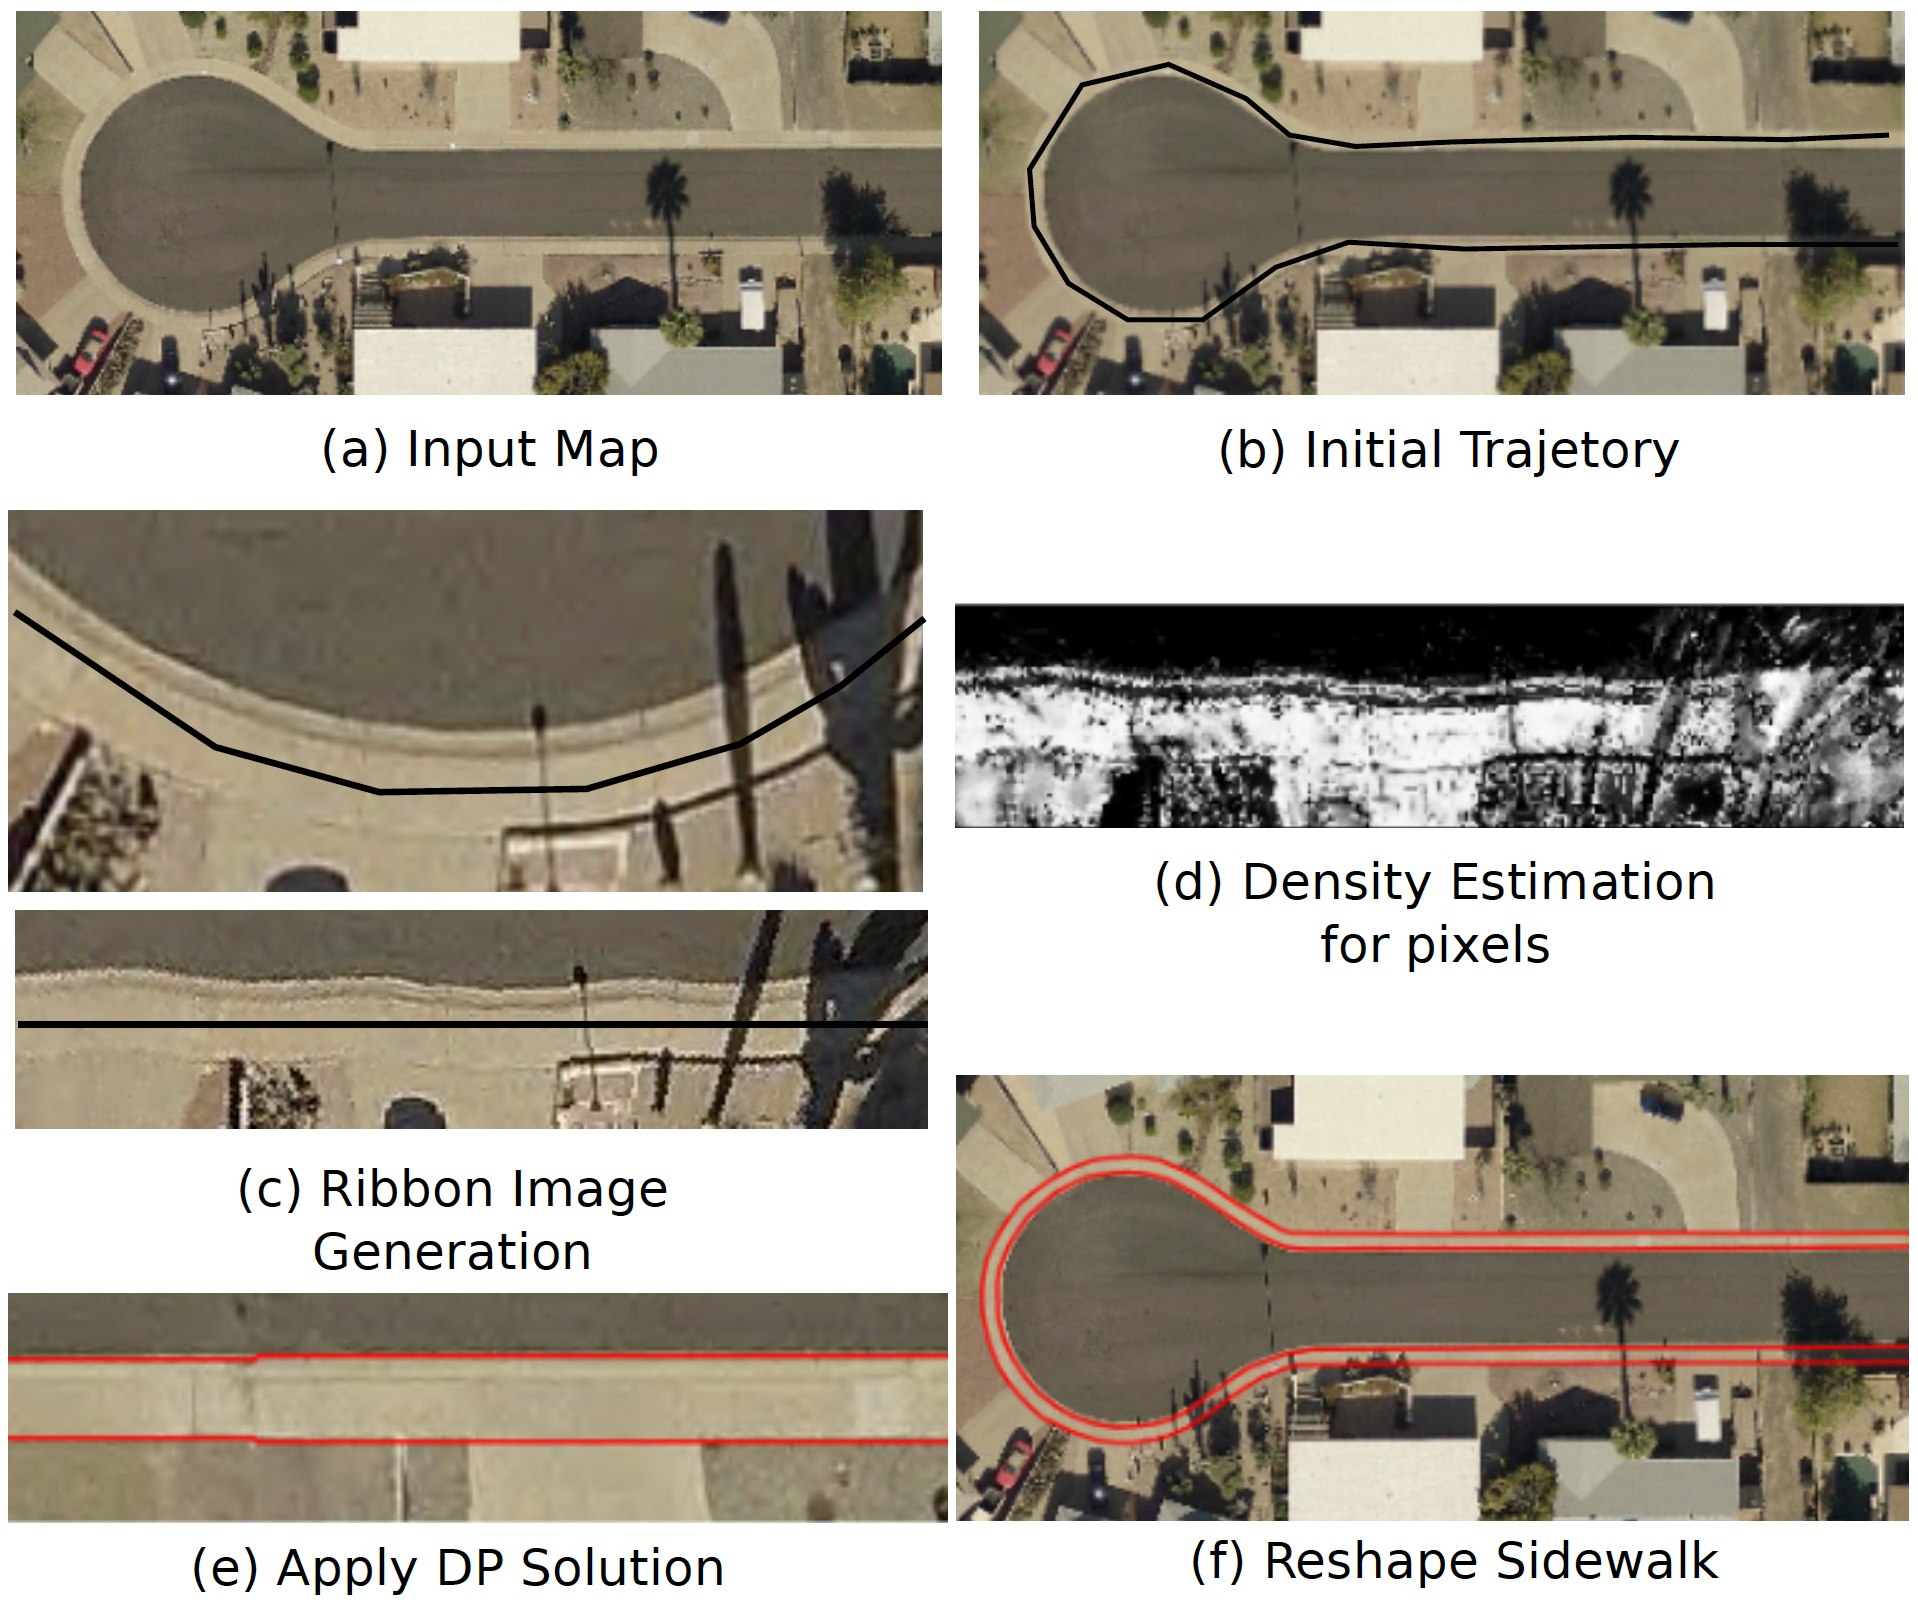
\includegraphics[width=0.9\textwidth]{Figures/diagram.png}
\caption[Framework Overview 2]{Our approach adopted to predict precise boundaries for ribbon-like features. Where black line indicated a sidewalk's geometric information, and red lines shown our result for the sidewalk boundaries. From (a) to (f), the 6 step approach introduce input map (a), initial trajectory (b), ribbon image generation (c), density Estimation for pixels(d), apply \ac{DP} solution(e), reshape sidewalk(f).}
\label{fig:Apparatus}
\end{center}
\end{figure}

\section{Warping an input image}

We take as input an image $\InputImage{}$ and a trajectory $\InputTrajectory{}=\langle \vec{p}_0, \vec{p}_1,\dots,\vec{p}_m\rangle$ where each $\vec{p}_i=(x_i, y_i)^T$ is a point on the initial estimate of a ribbons trajectory (re-sampled and smoothed). Further, we are able to estimate unit-length tangent vectors $\vec{u}_i$ and their perpendiculars $\vec{v}_i$; for example by using the secant method 
\begin{align}
  \vec{u}_i &= \frac{\vec{p}_{i+1}-\vec{p}_{i-1}}{\|\vec{p}_{i+1}-\vec{p}_{i-1}\|} \\
  \vec{v}_i &= \left(\begin{array}{cc}
       0  & 1 \\
       -1 & 0
  \end{array} \right) \vec{u}_i
\end{align}
where the endpoints are repeated. We define the warped ribbon-image $\RibbonImage{}$ so that $\RibbonImage{[i,j]}=\InputImage{}(\vec{p}_i+ j \vec{v}_i)$. We use the convention that square-brackets to indicate discrete indices and rounded parenthesis indicate interpolated samples.  An example of the process is shown in \figref{fig:Sample_Sidewalk_4} and \figref{fig:Apparatus}(c). 

\begin{figure}
    \centering
    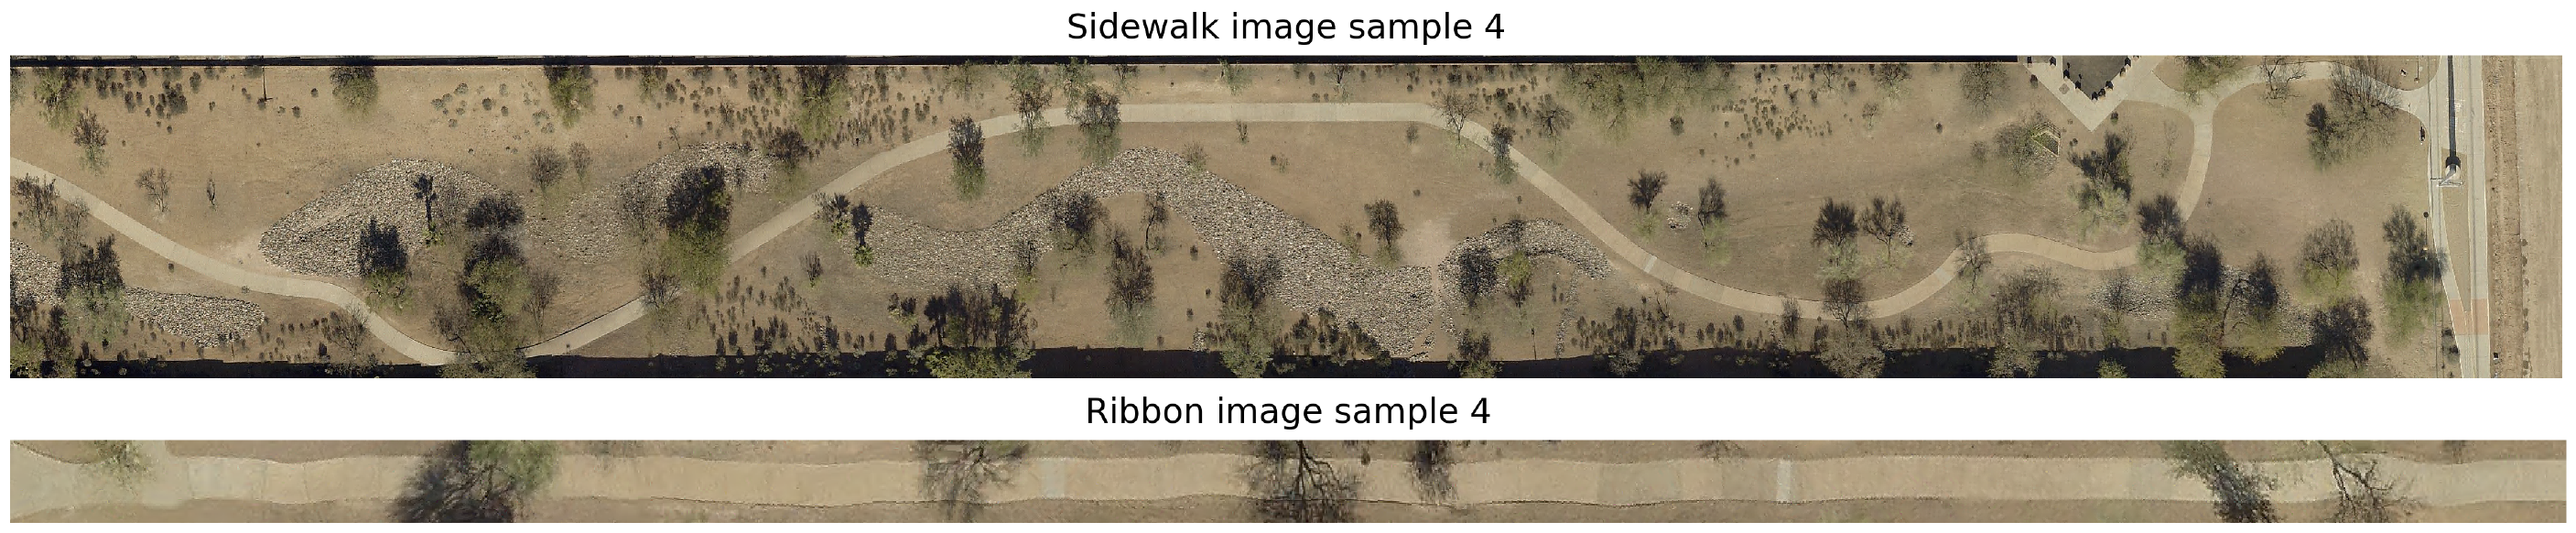
\includegraphics[width=\textwidth]{Figures/Sample4_needed.png}
    \caption[Sample Sidewalk 1]{A ribbon image straighten output which used the previous process from figure \ref{fig:StraightenProcess} to convert an original image into ribbon image .}
    \label{fig:Sample_Sidewalk_4}
\end{figure}

% \begin{figure}[ht]
%     \centering
%     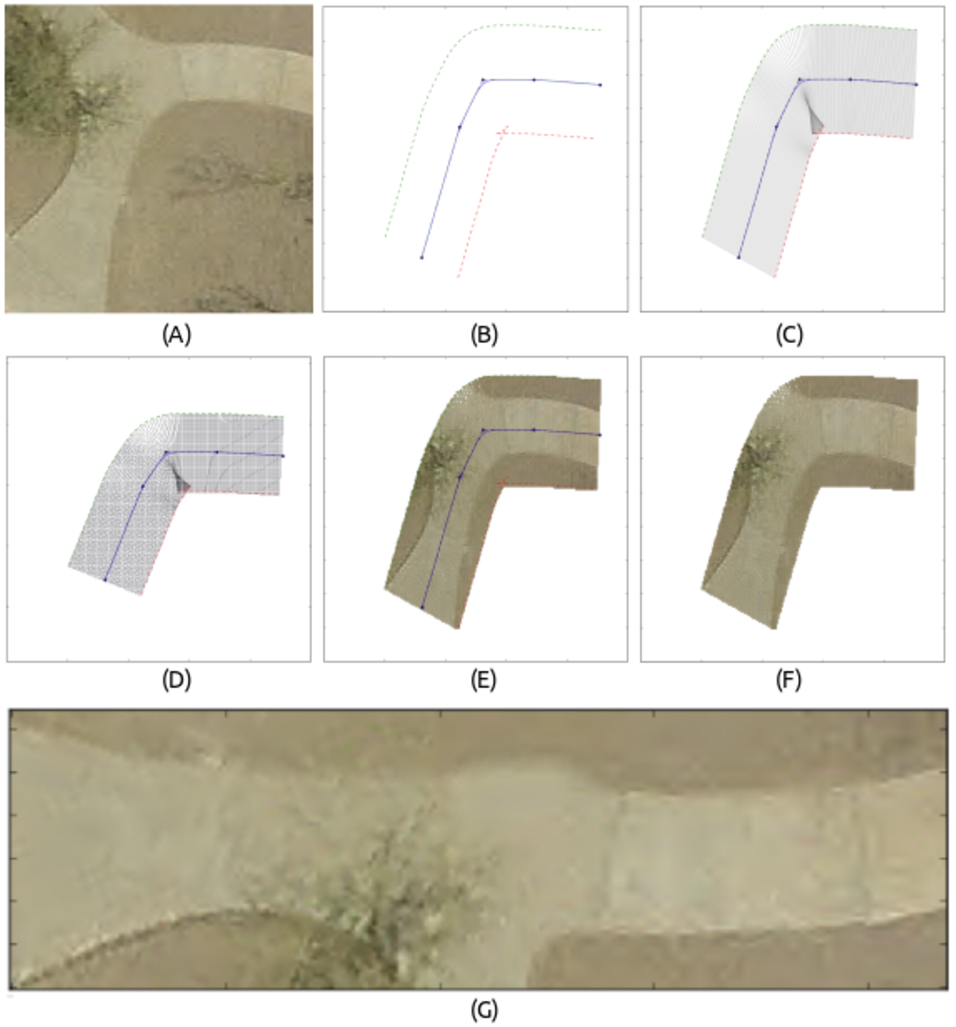
\includegraphics[width=0.95\columnwidth]{Figures/straghten.pdf}
%     \caption[Ribbon Image Generation]{Ribbon image generating process: (a) raw input $\InputImage{}$, (b) we densely resample and smooth the trajectory using $\MaxRadius{}$ iterations of Laplacian smoothing and show the locations of warped pixels of $\RibbonImage{}$ within $\pm \MaxDistance{}$;  (c) the warped ribbon image $\RibbonImage{}$ shown in the original reference frame and  (d) the generated the ribbon image (shown transposed to fit in the figure).}
%     \label{fig:StraightenProcess}
% \end{figure}

% \begin{figure}[ht]
%     \centering
%     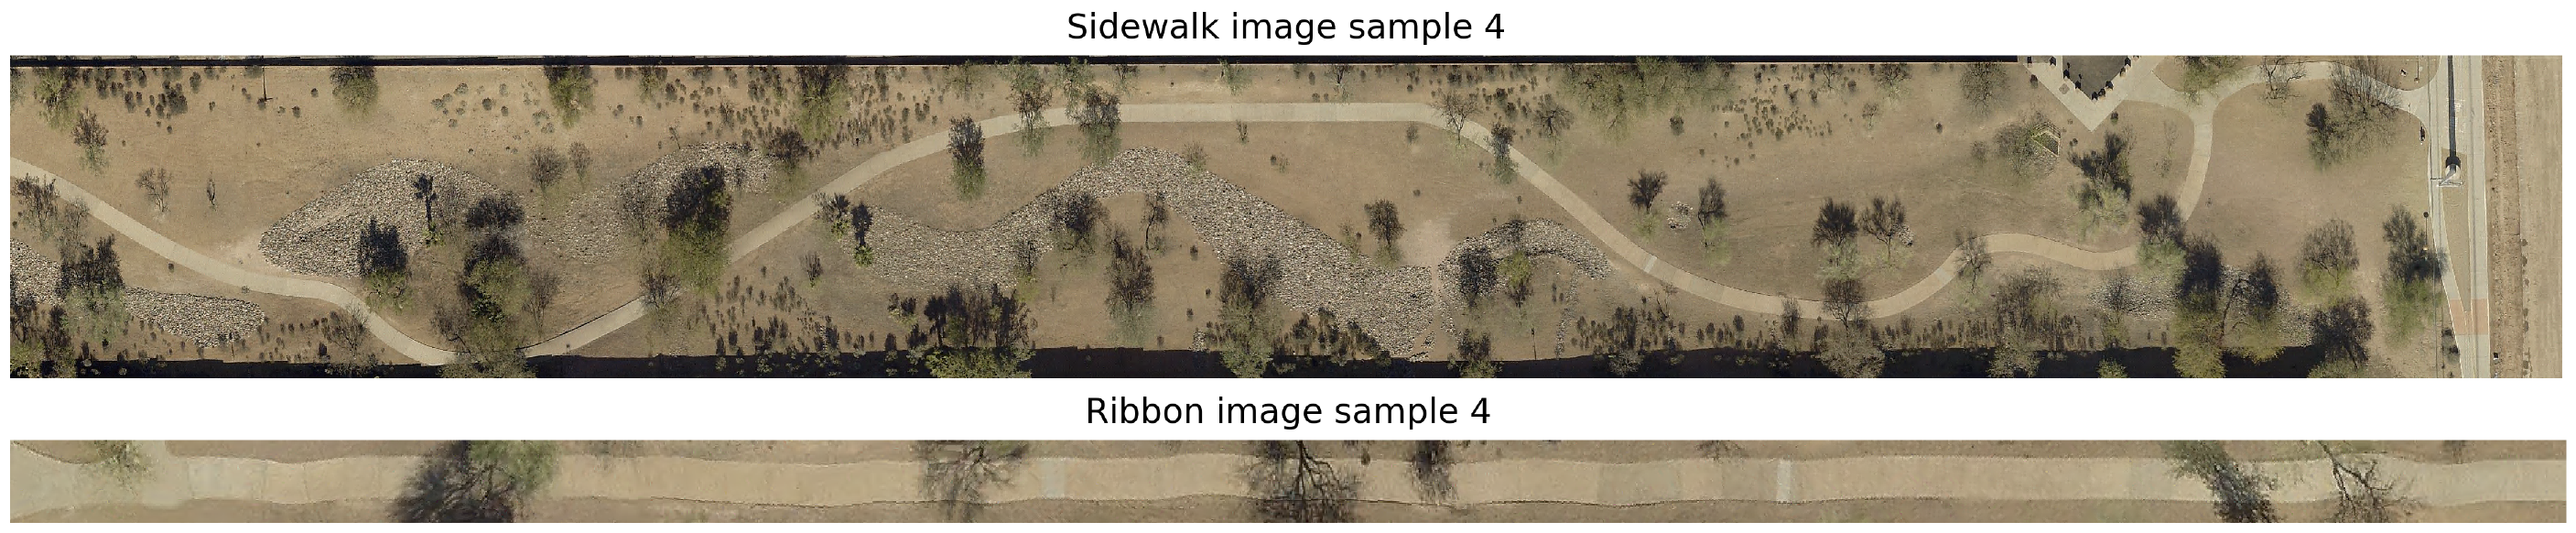
\includegraphics[width=0.95\columnwidth]{Figures/Sample4_needed.png}
%     \caption[Sample Sidewalk]{A ribbon image; the original image $\InputImage{}$ (top) was warped so that the trajectory is a straight line to create a ribbon image $\RibbonImage{}$ (bottom), shown transposed.}
%     \label{fig:Sample_Sidewalk_4}
% \end{figure}

\section{Density Estimation}
We aim to find a new trajectory $\OutputTrajectory{[0\dots m]}$ and radius $\OutputRadius{[0\dots m]}$ that are most likely given an input image. We first must estimate the probability of observing a color within the ribbon.  
Given an input image $\RibbonImage{}$, let $\Pr(\text{pos}|\phi,\theta)$ denote the probability that a pixel is a part of a ribbon given an observed color $\phi$ and set of learnable parameters $\theta$. 
We aim to estimate parameters $\theta$ that maximize the likelihood of our \textit{initial} path. 

\begin{figure}[H]
    \centering
    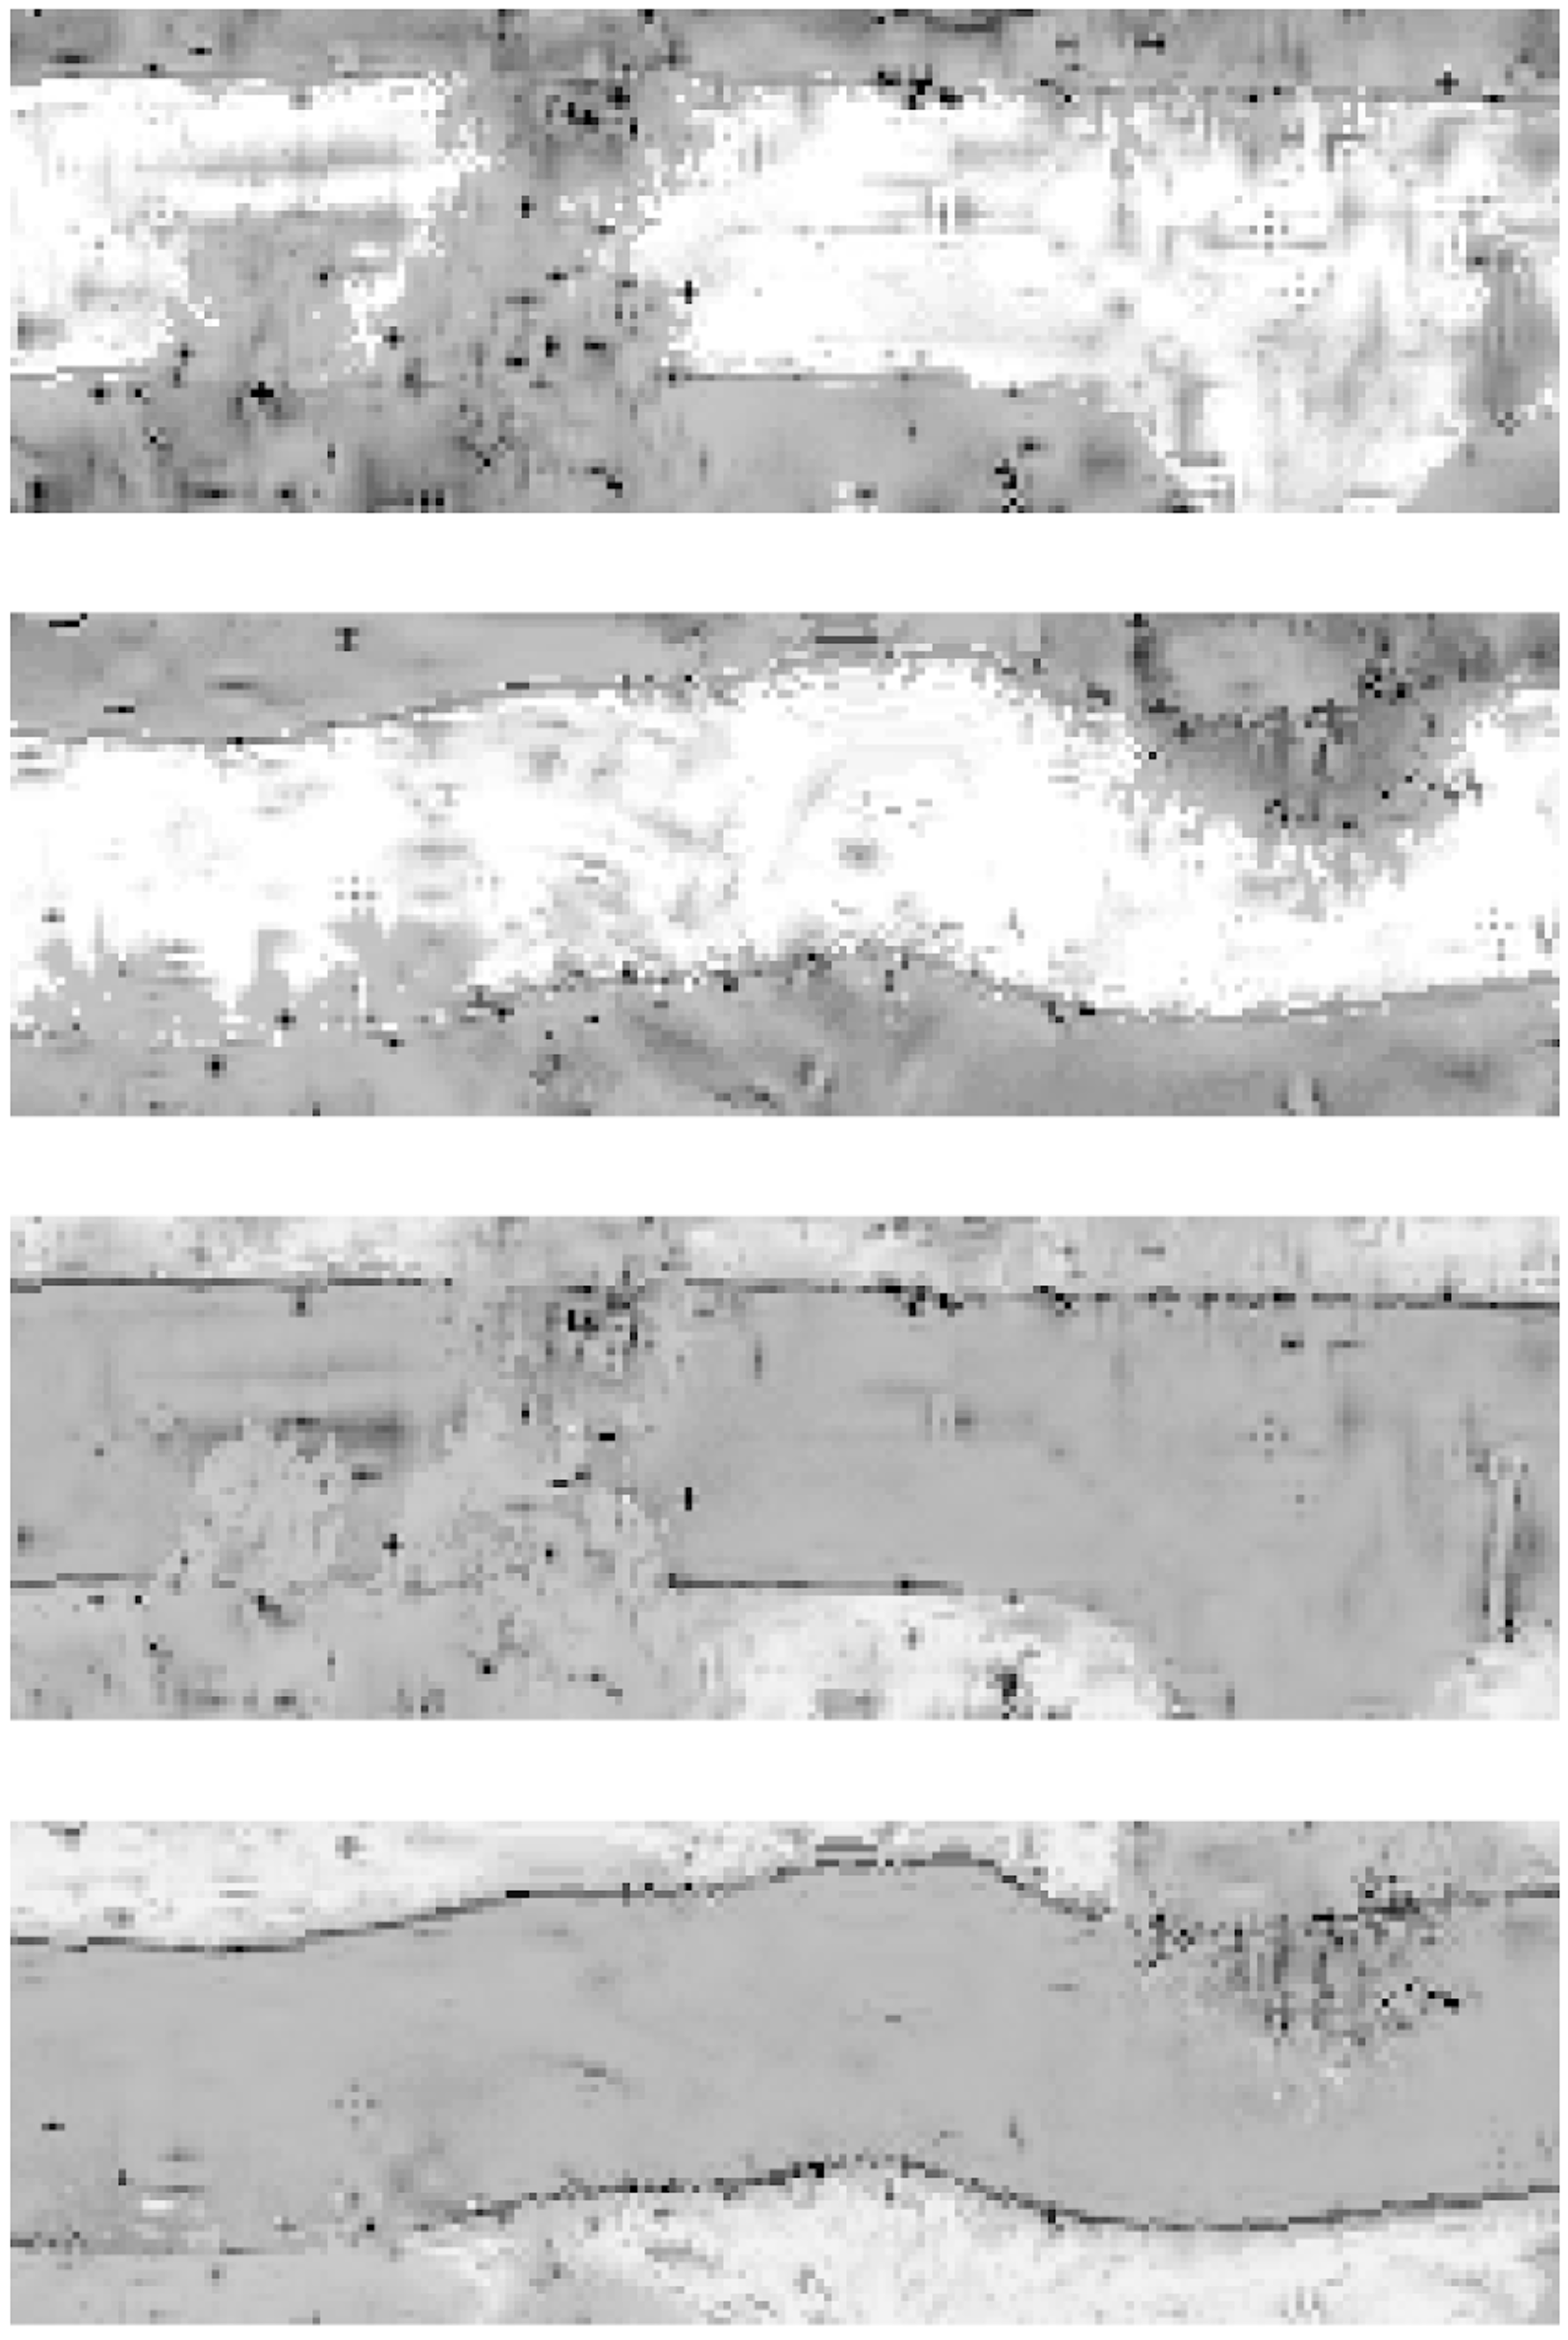
\includegraphics[width=0.75\columnwidth]{Figures/GMM_sample6.png}
    \caption[\ac{GMM} Result 2]{Example of GMMs on sample sidewalk. Row 1 and 2 shows the foreground GMM for sample sidewalk, and row 3 and 4 shows the back-ground for simple sidewalk. We use grey-scale to show the changes of probabilities, where for foreground, white is more likely to be sidewalk, and black is not.}
    \label{fig:GMM_result_2}
\end{figure}

We do not in general have a reliable estimate for the initial radius of our ribbon, 
but we can construct a trimap (\figref{fig:ribbon_3d_2}, bottom), as is done by \GrabCut{}, in order to estimate $\theta$. We choose a distance $\MaxDistance$ and numbers $\MinRadius < \MaxRadius$ 
so that all pixels with a distance of $[0, \MinRadius)$ are likely part of the ribbon (positive), all pixels within a distance of $[\MinRadius, \MaxRadius)$ are unknown, and others are are assumed not to be part of the ribbon (negative); 
In our experiments we chose  $\MaxRadius$ as twice the expected mean width of ribbons (e.g. 2 meters), $\MinRadius = \MaxRadius/2$, and $\MaxDistance=\MaxRadius+\MinRadius$.  
In figure \ref{fig:ribbon_3d_2} these regions correspond to strips of pixels in $\RibbonImage{}$ along the edges and center of the image.

% \begin{figure}[h!]
%     \centering
%     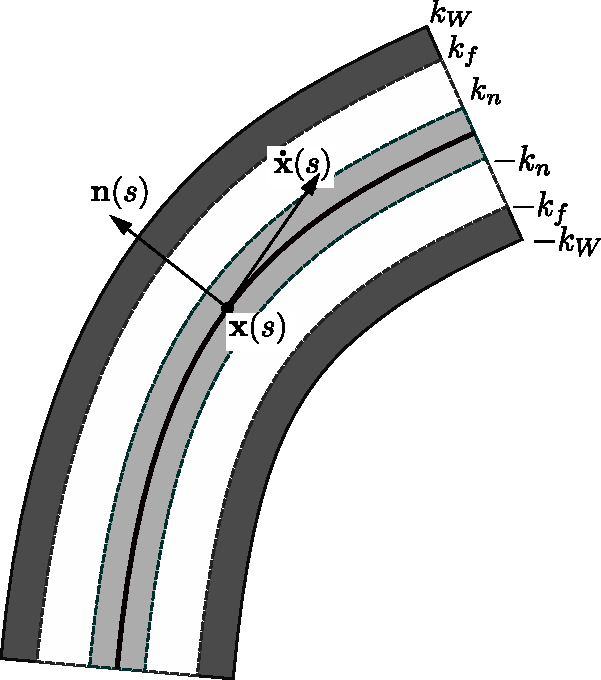
\includegraphics[width=0.3\textwidth]{Figures/sw-figure.pdf}
%     \caption[2D Ribbon Image]{A demonstration of the parameters for a ribbon in 2D, where $k_n$ indicates a lower-estimate for the radius of the ribbon, $k_f$ is an upper estimate, and $k_W$ is the maximum width of the ribbon image.}
%     \label{fig:2d_ribbon}
% \end{figure}

We use the EM-GMM algorithm to find a max-likelihood estimate of $\theta$ as a pair of Gaussian mixtures so that $\Pr(\phi|\text{pos}, \theta)$ is a mixture of four multivariate Gaussian functions and $\Pr(\phi|\text{neg}, \theta)$ is a mixture of eight; then $\Pr(\text{pos}|\phi, \theta)$ can easily be found using Bayes theorem as 
$$\Pr(\text{pos}|\phi, \theta)= \frac{\Pr(\phi|\text{pos}, \theta)}{\Pr(\phi|\text{pos}, \theta)+\Pr(\phi|\text{neg}, \theta)}.$$



%\FloatBarrier

The resulting probabilities are illustrated in \figref{fig:GMM_result_2}; we observe that even a coarse initial trajectory is usually enough to learn a more detailed, but noisy, estimate for the foreground object shape. However colors alone are not able to discriminate between occlusion and camouflage regions (such as the driveway in \figref{fig:GMM_result}). For rotational convenience we let $p[i,j]=-\lg \Pr(\text{pos}|\RibbonImage{}[i,j], \theta)$ and $q[i,j]=-\lg \Pr(\text{neg}|\RibbonImage{}[i,j], \theta)$; then the \ac{NLL} of a ribbon is proportional to a sum of $p[i,j]$ for all $i,j$ within the ribbon and $q[i,j]$ for all $i,j$ outside the ribbon. The aim of our \ac{DP} solution is to simultaneously optimize the probability based on color and shape of a ribbon-like feature. 


\section{A Dynamic Programming Algorithm}

\begin{figure}[htb]
    \centering
    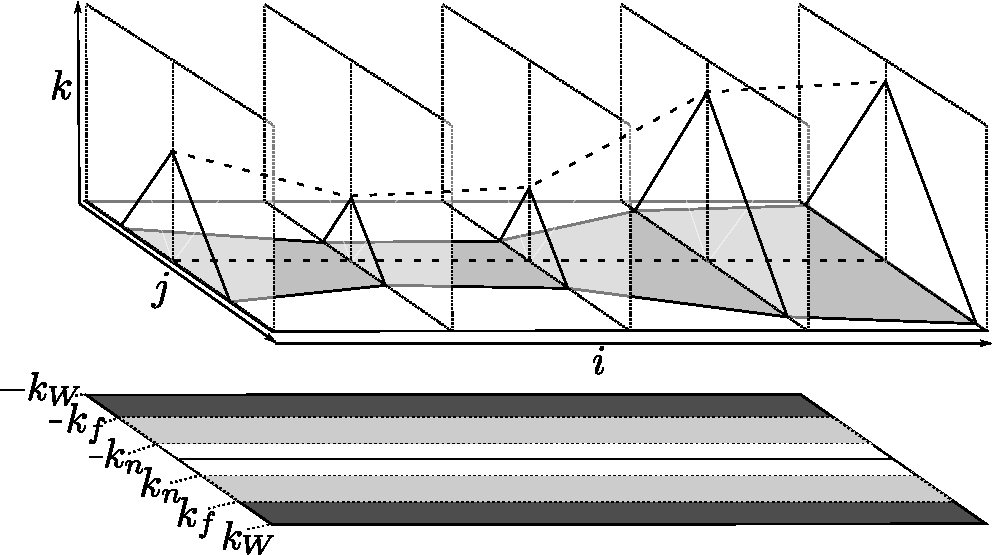
\includegraphics[width=0.95\columnwidth]{Figures/ribbon-3d-combined.pdf}
    \caption[3D Ribbon Image 2]{An illustration of the parameters for a ribbon: (top) the $k$ axis captures the thickness of the ribbon and the $i$ axis captures the distance along the initial ribbon, the $j$ axis records horizontal displacements from the initial ribbon's medial curve; (bottom) the boundaries of the ribbon must lie within $\pm \MaxDistance{}$, pixels within $\pm \MinRadius{}$ of the center are probably part of the ribbon and pixels further than $\pm \MaxRadius{}$ are likely negative. }
    \label{fig:ribbon_3d_2}
\end{figure}

We take $\RibbonImage{}$ as an input ribbon image with $m$ rows and $n=2\MaxDistance+1$ columns; $\RibbonImage{}{[i,j]}$ is a pixel in the image. We have an estimate $\Pr(\text{pos}|\RibbonImage{}_{[i,j]}, \theta)$ which we abbreviate as $p_{[i,j]})$. In addition there is some small set of allowed perturbations $\delta=\{(\delta_j, \delta_k)\}$ where $\delta_j$ is a change in direction and $\delta_k$ is a change in the radius of the ribbon. Each perturbation has a probability $\Pr(\delta_j, \delta_k)$ that controls the shape of the curve; in our experiments we use $\delta_j\in\{-1,0,1\}, \delta_k\in\{-1, 0,1\}$ in order to ensure that results are connected, and  $\Pr(\delta_j, \delta_k)=\Pr(|\delta_j|)\Pr(\delta_k)$ is two independent multinomial distributions which require only three parameters due to symmetry and because probabilities sum to unity. We can interpret $c_\mathit{bend}=-\lg \Pr(\delta_j=\pm1)$ as a penalty for bending the curve, and $c_\mathit{shrink}=-\lg \Pr(\delta_k=-1)$ as a penalty for shrinking the radius, or $c_\mathit{expand} = -\lg \Pr(\delta_k=1)$ as a penalty for expanding the radius of the curve. 

We visualize the problem of finding a ribbon as one of choosing a three-dimensional path through a scale-space where the first two dimensions represent locations of the ribbon's center, and the third dimension represent the thickness of the ribbon as illustrated in \figref{fig:ribbon_3d}. Every ribbon must start at one end of the image and follow a three-dimensional path through scale-space to reach the other end one slice at a time. Each slice corresponds to a row of the ribbon image and a point at location $(j, k)$ in the slice partitions the row into negative regions $(0\twodots{}j-k-1)$ and $(j+k+1\twodots{}n)$ with a positive region at $(j-k \twodots{} j+k)$ with thickness $2k+1$. The likelihood of any location $(j, k)$ is the product of the probabilities that each pixel on the same row belongs to the corresponding positive or negative regions.  In fact the probability is exponentially related to the size of each pixel; if one were to increase the resolution by a factor of $r$ then the contribution of each pixel would be raised to the power of $\frac{1}{r}$ so that the product would stay constant. In order to make our parameters invariant to scale, we divide the \ac{NLL} by $\MaxDistance{}$ when estimating the likelihood of a given $(j,k)$. 

We model the probability of a ribbon as the product of the probability of each location $(i, j, k)$ along the path times the probability of each edge from slice $i$ to slice $i+1$. We use dynamic programming to search to a path that minimizes the \ac{NLL} (the cost) of a path in procedure \proc{Segment-Ribbon}.

The pseudocode can be interpreted as follows: Line \ref{li:loop-slices} iterates through each slice of the ribbon image. Line \ref{li:loop-radius} iterates through all possible radii and line \ref{li:loop-center} explores all possible ribbon-centers from left to right. We use a variable $s$ to calculate \ac{NLL} of a set of regions as the ribbon shifts from left to right. If this is not the first slice, then line \ref{li:min-from-pred} selects the least-expensive (most probable) path that leads to location $(i, j, k)$ in the scale space.  At each step on pixel toggles from negative to positive, and one toggles from positive to negative as $s$ is updated in line \ref{li:update-s}.  We return the costs as well as the final offset and scale $(j^*, k^*)$ of the best path. 


\begin{codebox}
\Procname{$\proc{Segment-Ribbon}(\RibbonImage{})$} \label{alg:segmet-ribbin}
\li $p[i,j]\gets -\lg \Pr(\RibbonImage{}[i,j])/\MaxDistance{}$, 
          \hspace{2ex} $q[i,j] \gets -\lg \Pr(1-\RibbonImage{}[i,j])/\MaxDistance{}$
\li $C{[0\twodots{}m, 0\twodots{}n, 0\twodots{}n]} \gets \infty$
\li \For{$i \gets 0 \To m$} \Do                                                \label{li:loop-slices}
\li     \For $k \gets 0 \To \lfloor n/2 \rfloor $ \Do                          \label{li:loop-radius}
\li         $s = \displaystyle{\sum_{j=0}^{2k} p[i,j] +\sum_{j=2k+1}^n  q[i, j] }$
\li         \For $j \gets k \To n-k$ \Do  \label{li:loop-center}
\li              \If $i > 0$  \Do                                              \label{li:if-has-pred}
\li              $v \gets s {+}\displaystyle{\min_{\delta_j, \delta_k}\left(  
                              \begin{aligned}
                              C[i{-}1,j{+}\delta_j,k{+}\delta_k] \hspace{3ex}\\
                              \hfill{}-\lg \Pr(\delta_j, \delta_k)
                              \end{aligned}
                            \right)}$  
                               \label{li:min-from-pred}
\li              \Else $v\gets s$
                 \End
\li              $C{[i, j, k]} \gets v$                                       \label{li:dp-store}
\li              $s \gets s{+}q[i,j{-}k]{-}p[i, j{-}k]{+}p[i, j{+}k]{-}q[i,j{+}k]$ \label{li:update-s}
           \End
       \End
    \End
\li $j^*, k^* \gets \displaystyle{\arg\min_{j,k} C{[m, j, k]}}$
\li \Return $C, j^*, k^*$
\end{codebox}

The \proc{Backtrack-Ribbon} algorithm selects the least-costly (most probable) ribbon and it is copied into to $T$ and $R$; so that the most likely path has scale-space coordinates $(i, T[i], R[i])$ for $i=0\twodots{}m$. 



\begin{codebox}
\Procname{$\proc{Backtrack-Ribbon}(C, j^*, k^*)$} \label{alg:backtrack-ribbon}
\li $T{[0{\twodots}m]} \gets 0$, \quad $R{[0{\twodots}m]} \gets 0$             
\li $T{[m]}, R{[m]} \gets j^*, k^*$ \label{li:backtrack-best-last}
\li \For $i \gets m-1 \Downto 0$ \Do
\li      $\delta_j, \delta_k = \displaystyle{\arg\min_{\delta_j,\delta_k}C{[i,j{-}\delta_j,k{-}\delta_l]}{-}\lg \Pr(\delta_j,\delta_k)}$
\li      $T{[i]}, R[i] \gets T{[i+1]}-\delta_j, R{[i+1]}-\delta_k$                                                 \label{li:backtack-choose-pred}
    \End
\li \Return $T, R, C_{[m, j^*, k^*]}$
\end{codebox}


If one wishes the path to be connected in scale-space, then there are only $3\times3$ possible values for $\delta_j, \delta_k$ in line \ref{li:min-from-pred}; so the algorithm is $\Theta(m n^2)$ and used $O(m n^2)$ space, where $m$ is the length of a ribbon and $n=2\MaxDistance+1$ is the maximum thickness of a ribbon. Since $\MaxDistance$ is typically a constant, this algorithm is effectively linear on the length of a ribbon.